\documentclass[letterpaper, 12pt]{article}
\usepackage[letterpaper, top=2.5cm, bottom=2.5cm, left=3cm, right=3cm]{geometry} %margenes
\usepackage[utf8]{inputenc} %manejo de caracteres especiales
\usepackage[spanish]{babel} %manejo de encabezados de inglés a español
\usepackage{fancyhdr} %formato de los encabezados de página
\usepackage{ragged2e} %alineado real justficado
\usepackage{graphicx} %manejo de imagenes
\usepackage{amsmath} %manejo de notación matemática
\usepackage{mathtools} %manejo de notación matemática
\usepackage{blindtext} %texto de relleno
\usepackage{cancel} %permite la simbolización de cancelación de terminos
\usepackage{enumitem}[shortlabels] %listas con letras
\usepackage{amssymb} %manejo de simbolog►1a matematica

\pagestyle{fancy}
\fancyhf{}
\rfoot{\thepage}

\setlength{\abovedisplayskip}{0pt}
\setlength{\belowdisplayskip}{0pt}

\begin{document}

\setcounter{page}{1}
\thispagestyle{fancy}
\lhead{\textbf{Tarea 1, U1}}
\rhead{\textbf{17/09/2020}}
\section{Vectores en el espacio}
\subsection*{Graficar y calcular la magnitud de \(\vec{AB},\,\vec{CB},\,\vec{DC},\,\vec{AD},\,-\vec{AD}\) dados los sig. puntos:}
\begin{itemize}
    \item \(A=(1,3)\)
    \item \(B=(6,-2)\)
    \item \(C=(2,-4)\)
    \item \(D=(-3,-1)\)
\end{itemize}

\subsubsection*{-Gráfica de los vectores}    
\centering
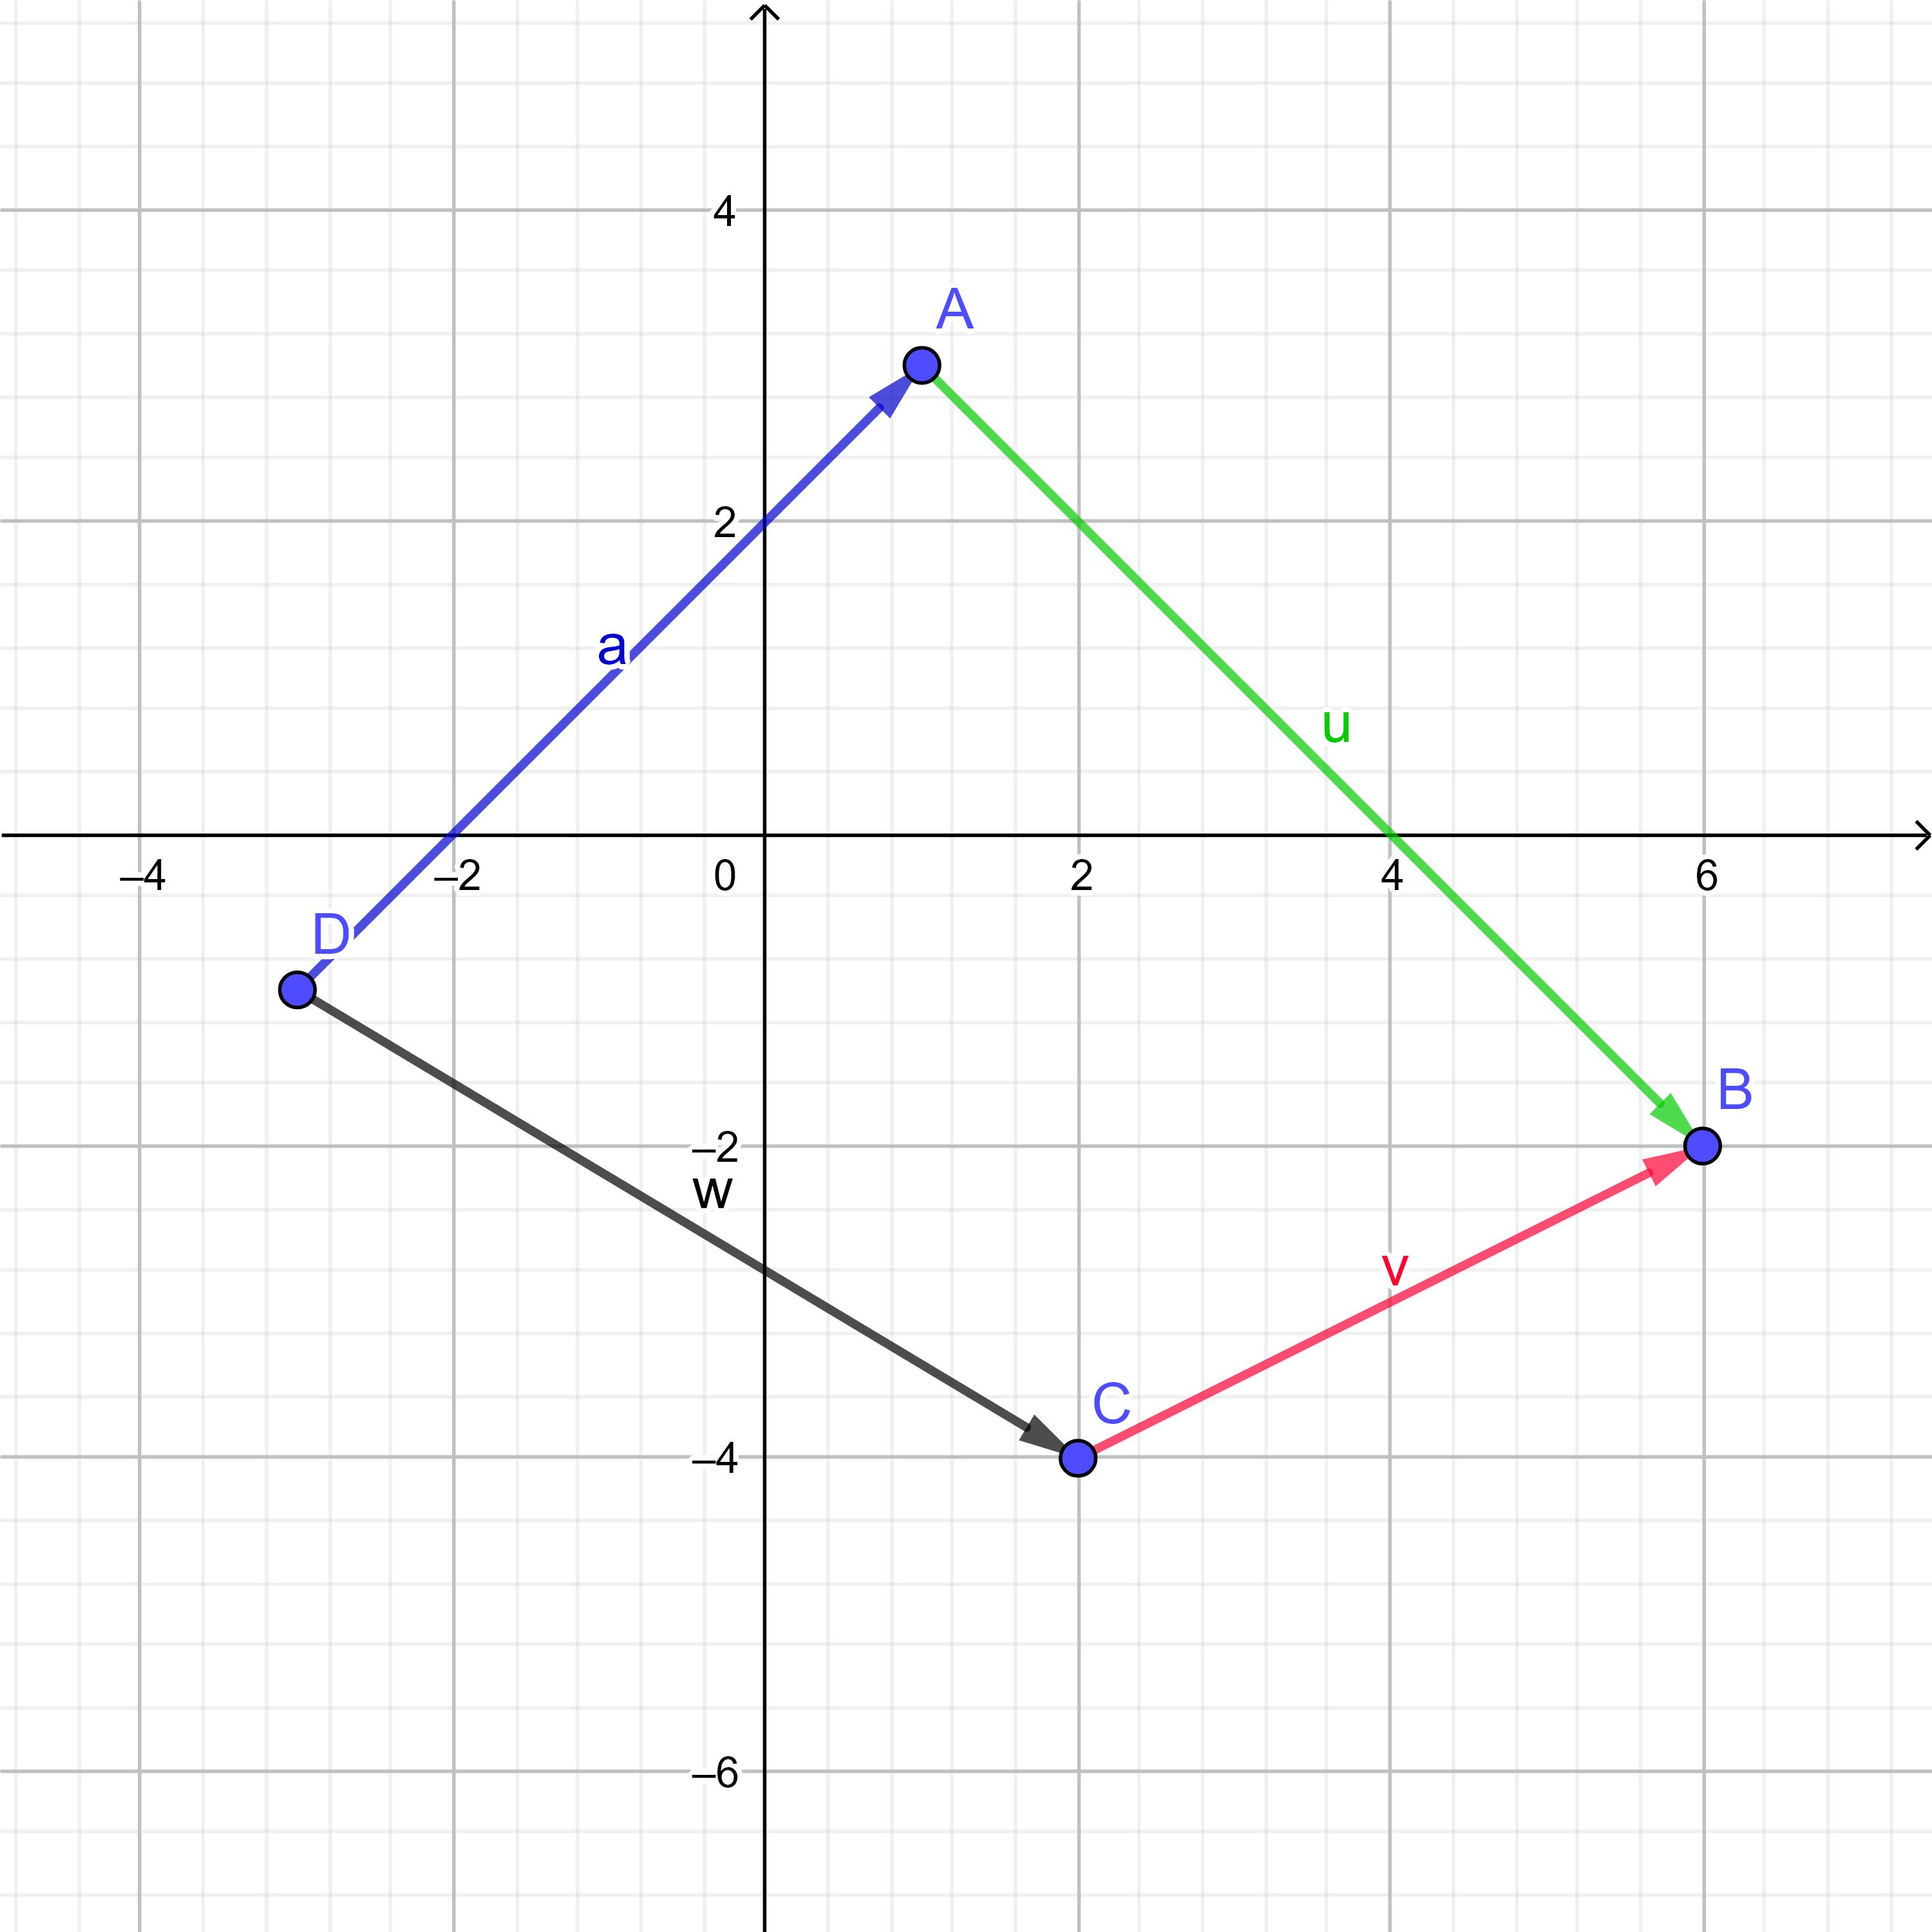
\includegraphics[width=15cm]{graficasT1U1.png}
\justify
\subsubsection*{-Magnitudes}
\begin{justify}
\textbf{*Magnitud \(\vec{AB}\):}
\justify
Como estamos manejando un vector compuesto de dos puntos, procederemos a utilizar la sig: formula (la cual se aplicara en las magnitudes restantes):
\[d=\sqrt{(y_2-y_1)^2+(x_2-x_1)^2}\]
La cual se deriva por aplicar el Teorema de Pitagoras.
\begin{align*}
\|\vec{AB}\|&=\sqrt{(y_2-y_1)^2+(x_2-x_1)^2}\\
\|\vec{AB}\|&=\sqrt{(-2-3)^2+(6-1)^2}\\
\|\vec{AB}\|&=\sqrt{(-5)^2+(5)^2}\\
\|\vec{AB}\|&=\sqrt{25+25}\\
\|\vec{AB}\|&=\sqrt{50}
\end{align*}

\justify
\textbf{*Magnitud \(\vec{CB}\):}
\begin{align*}
    \|\vec{CB}\|&=\sqrt{(y_2-y_1)^2+(x_2-x_1)^2}\\
    \|\vec{CB}\|&=\sqrt{(-4+2)^2+(2-6)^2}\\
    \|\vec{CB}\|&=\sqrt{(-2)^2+(-4)^2}\\
    \|\vec{CB}\|&=\sqrt{4+16}\\
    \|\vec{CB}\|&=\sqrt{20}
\end{align*}

\justify
\textbf{*Magnitud \(\vec{DC}\):}
\begin{align*}
    \|\vec{DC}\|&=\sqrt{(y_2-y_1)^2+(x_2-x_1)^2}\\
    \|\vec{DC}\|&=\sqrt{(-1+4)^2+(-3-2)^2}\\
    \|\vec{DC}\|&=\sqrt{(3)^2+(-5)^2}\\
    \|\vec{DC}\|&=\sqrt{9+25}\\
    \|\vec{DC}\|&=\sqrt{34}
\end{align*}

\justify
\textbf{*Magnitud \(\vec{AD}\):}
\begin{align*} 
    \|\vec{AD}\|&=\sqrt{(y_2-y_1)^2+(x_2-x_1)^2}\\
    \|\vec{AD}\|&=\sqrt{(-1-3)^2+(-3-1)^2}\\
    \|\vec{AD}\|&=\sqrt{(-4)^2+(-4)^2}\\
    \|\vec{AD}\|&=\sqrt{16+16}\\
    \|\vec{AD}\|&=\sqrt{32}
\end{align*}

\justify
\textbf{*Magnitud \(-\vec{AD}\):}
\justify
Debido a que una magnitud no es afectada por cambios de signos de sus parámetros, podemos decir que: \(\|\vec{AD}\|=\|-\vec{AD}\| \therefore \|-\vec{AD}\|=\sqrt{32}\).
Esto pasa debido a que la multiplicación escalar de \(-1\) a un vector cualquiera solo hara que apunte en dirección contraria, por lo que sus valores solo cambiaron de dirección, resultando
en el mismo valor de magnitud que su homologo positivo.
\end{justify}
\end{document}